\chapter{A selection of methods for change point detection}\label{chp:3}

\minitoc

\clearpage

%Although the recommendations for the use of the substances are formulated in the marketing authorization issued by ANSES \citep{ephy}, their practical use is not subject to control by the Agency. Cultivation practises depend on meteorological conditions and professional habits. This partly explains the spatio-temporal heterogeneity presented in Section \ref{chp:2:3}. Our aim is to find homogeneous time periods and geographical areas and to perform a statistical comparison of these regions in these stable periods to support the expert analysis. 
%In this chapter we focus on the identification of stable temporal patterns using segmentation methods. This mathematical area is covered by several surveys \citep{truong2020,basseville1993detection,bardet2020}. More specifically, we have focused on certain types of methods that seem suitable for the application domain of phytopharmacovigilance, namely change point detection methods. Moreover, this work will focus only on the offline methods that we will develop in the following sections. This choice was motivated by the speed of data collection and storage of data on pesticide concentrations. Nevertheless, for readers who wish to refer to it, we can state that there is no shortage of online detection methods in the literature \citep{liu2017change,Li2021,hohle2010online,ranganathan2010pliss,li2015m}.
%This chapter is structured as follows: Section \ref{chp:3:1} presents a classical modelling of change-point detection and explores the different ways to evaluate temporal sub-signals; Section \ref{chp:3:2} provides methods to estimate the number of change-points in a signal and their position; Section \ref{chp:3:3} gives an efficient way to obtain different results of segmentations; Section \ref{chp:3:4} searches for application of change- point detection methods to data that have the same characteristics as in Section \ref{chp:2:3}.

%First, we want to detect homogeneous temporal periods in a monitored substance use. 
%of pesticide concentrations
%for readers who wish to refer to it, we can state that there is no shortage of on-line detection methods in the literature \citep{liu2017change,Li2021,hohle2010online,ranganathan2010pliss,li2015m}.
%how 

Let us recall that our first objective is the detection of homogeneous temporal periods in the use of a chemical substance for which monitoring data is available. This task can be viewed as a change point detection problem, where the change points delineate homogeneous time intervals. In this chapter, we propose to go over some available methods to solve this problem.  

We have chosen to limit this chapter to off-line methods, i.e. methods that search for changes in known features of fully acquired signals. This choice is motivated by the speed of data collection and storage in the context of pesticide concentration monitoring, as these data are not collected in real time. Nevertheless, for the sake of completeness, we can mention that there exist quite a number of on-line detection methods in the literature \citep{liu2017change,Li2021,hohle2010online,ranganathan2010pliss,li2015m}.This present thesis draws on the following research \citep{truong2020,basseville1993detection,bardet2020}. 

This chapter is structured as follows: Section \ref{chp:3:1} presents a classical modelling framework for change point detection and explores the different ways to evaluate temporal sub-signals; Section \ref{chp:3:2} presents existing methods for estimating the positions of a known number of changes; Section \ref{chp:3:3} reviews a selection of methods that have been proposed to estimate the number of change points when the latter is unknown; Section \ref{chp:3:4} reviews efficient available algorithms to obtain different segmentation results; Section \ref{chp:3:5} looks at applying change point detection methods to data that have the same characteristics as in Section \ref{chp:2:3}.

\section{Model and cost functions}\label{chp:3:1}

% We use the following convention, let 
% operate on 
% This function associates a cost to the segment it is evaluated on. 

We describe the most general framework for a change-point model. We consider a signal consisting of observations $\bm y = (y_1,...,y_n)$, which are the realisations of random variables $Y_1,...,Y_n$. The variables $Y_i$ are recorded sequentially, and the recording times are not necessarily equidistant. Integrating the irregular sampling times or the temporal gaps between the observations in the modelling is not in the scope of this survey. Thus, the indices in $Y_i$ are only indicators of the order of occurrence in the sample and not of the observation times. \\
Some characteristics (trend, mean, variance, etc...) of the signal $\bm y$ are supposed to change at the $K^*$ indices $\tau^*_1 <... < \tau^*_k <... < \tau^*_{K^*}$. Moreover, we set $\tau^*_0 = 0$ and $\tau^*_{K^*+1} = n$. The purpose of breakpoint detection is to estimate the positions $\tau^*_k$ and the number of breaks $K^*$ when they are unknown. We denote $y_{u:v}$ as a segment of the signal from the u-th coordinate to the v-th. The goal is to identify such segments in the data for which the characteristics mentioned above are stable. \\
According to the nomenclature proposed by \cite{truong2020}, change point detection methods are based on a cost function $W$ for individual segments. Intuitively, when the properties (on which changes are investigated) of the segment $y_{u:v}$ are homogeneous, the cost $W(y_{u:v})$ takes low values. The total cost $\CC(\bm y,\TT)$ associated with a segmentation $\TT = (\tau_{k})_{k=1}^K$ with $K$ change points is given as the sum of the costs of all segments:
%We define, for any $y_{u:v}$, $\TT = \{\tau_1,\dots,\tau_K\} \subset \{u,\dots,v\}$ a set of ordered indices and $\lvert \TT \rvert$ its cardinal. Implicitly, we define $\tau_0 = u$ and $\tau_{K+1} = v$. Although this notation is often used for the full signal $\bm y$, we will always indicate the data segment from which $\TT$ is drawn in the parameters of the functions using the notation $\TT$.
\begin{equation}\label{chp:3:costfunc}
\CC(\bm y,\TT) = \sum_{k=0}^{\lvert \TT \rvert} W(y_{\tau_k+1:\tau_{k+1}}), 
\end{equation}     

With these notations and assuming $K^*$ is known, finding the change points is equivalent to solving the optimization problem:

\begin{equation}\label{chp:3:optKknown}
 \widehat{\TT}  = \arg \min_{\lvert \TT \rvert = K^*}  \CC(\bm y, \TT) = \arg \min_{\lvert \TT \rvert = K^*} \sum_{k=0}^{K^*} W(y_{\tau_k+1:\tau_{k+1}})   
\end{equation}

The choice of the cost function $W$ determines the type of changes (in trend, mean, etc.) targeted by the detection. Figure \ref{fig:ex_cp} illustrates two different types of changes that may be of interest for change point detection. In the next parts of this section, we distinguish the cost functions according to the statistical inferences which they are based on, namely parametric or non-parametric inference. We give a non-exhaustive list of cost functions for each inference framework.

\begin{figure}[ht]
    \centering
    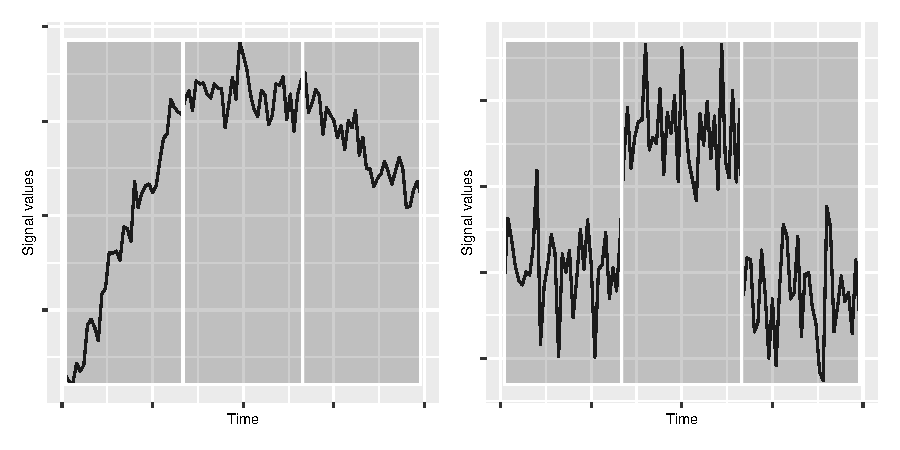
\includegraphics{figs/Chap2/Ex_CP_cost.pdf}
    \caption{Examples of types of change point detection. \\
    The figure on the left illustrates changes in trend: the data is simulated using a linear trend with a noise term following a normal distribution with known variance.\\
    The figure on the right illustrates changes in mean: the data follow a normal distribution with known variance and changes in mean.}
    \label{fig:ex_cp}
\end{figure}

\subsection{Parametric inference}

In the parametric case, the detection depends heavily on what we are looking for in the signal $\bm y$. For example, searching for slope changes in a signal \citep{Bai1994,Fearnhead2018} does not require the same modelling as detecting changes in the mean \citep{Frick2014,chen2012parametric}. We highlight these differences below.

A first classical cost function is based on the maximum likelihood estimation. In this setting, it is assumed that the observations located in the $k$-th segment follow a distribution $Q$ depending on a vector of parameters $\theta^*_k$ with $\theta_k \in \Theta$, a compact subset of $\mathbb{R}^p$. In other words, we suppose that all observations are sampled from the same distribution $Q$ but the values of $\theta^*_k$ change abruptly at each change-point $\tau^*_k$. 
More formally, we have that:
\begin{equation}
y_t \sim \sum_{k=0}^{K^*}f(.;\theta^*_k)\mathbbm{1}_{\tau^*_{k}+1\leq t \leq \tau^*_{k+1}},
\end{equation}
with $f$ being the density function of distribution $Q$ and the observed signal $\bm y =\{y_1,\dots,y_n\}$ is composed of independent random variables. The cost function used to evaluate the segments in this context is the negative log-likelihood calculated using $\hat\theta_{ML}$, the maximum likelihood estimator of the segment parameter. Hence, for a segment $y_{u:v}$ with $u < v$, we can write:  
\begin{equation}
W(y_{u:v}) = -\sup_{\bm \theta \in \Theta} \sum_{i = u}^{v} \ln f(y_i; \bm \theta)
\end{equation}
This method would prove useful in the example presented in the right side of Figure \ref{fig:ex_cp}. Applying the maximum likelihood estimator on the mean of Gaussian distribution would provide satisfying results. Other distributions than the Gaussian were investigated \citep{Maidstone2016a,Frick2014} since it is not always well suited for data (especially concentrations data).  

Cost functions adapted for changes in trend rely on piecewise linear regression. We place ourselves in the simplest case where $\bm y$ is univariate response to observed covariates $\{x_t\}_{t=1}^n$ such that $x_t \in \mathbb{R}^p$. Observations located in the $k$-th segment are modelled as: % supposed can be written
\begin{equation}
y_t \sim \sum_{k=0}^{K^*}(x'_t\theta^*_k + \epsilon_t)\mathbbm{1}_{\tau^*_{k}+1\leq t \leq \tau^*_{k+1}},
\end{equation}   
where $\theta^*_k \in \mathbb{R}^p$ are the regression parameters and $\epsilon_t$ is the noise on the signal, assumed to be Gaussian with zero mean and known variance in this precise setting. The adapted cost function in this configuration uses the least squares estimation and is expressed as:
\begin{equation}
W(y_{u:v}) = \min_{\theta \in \mathbb{R}^p}\sum_{t=u}^v(y_t-x'_t\theta)^2
\end{equation}
This modelling is perfectly suited for the detection of the changes in the left example of Figure \ref{fig:ex_cp}. Note that it can be straightforwardly extended to signals with non gaussian noise.

\subsection{Non-parametric inference}

%The cost function for a segment can also be adapted for non-parametric statistical inference. 
%This is equivalent to running the test under the following assumptions: 

Cost functions for segments have also been formulated for the non-parametric framework. Several strategies have been developed in the literature over time. These include the non-parametric maximum likelihood method \citep{Zou2014,Einmahl2003}, kernel methods \citep{Harchaoui2008,li2015m}, and rank-based methods \citep{Pettitt1980,Wang2019}. We will focus on the latter because it was adapted for censored observations in \cite{lung2015}.  

Detecting a breakpoint in a signal can be done using a test statistic based on the ranks of the observations rather than their values. The rank of the ith observation is defined as $R_i = \sum_{j =1}^n\mathbbm{1}(Y_j < Y_i)$. Moreover, we note $\hat{F}_n(t) = \frac{1}{n}\sum_{i = 1}^n\mathbbm{1}(Y_i < t)$ the empirical cumulative distribution function (c.d.f.). The cost function is derived from the Wilcoxon/Mann-Whitney rank criterion. Indeed, finding a single breakpoint in the signal amounts to testing the following assumptions:
\begin{itemize}
  \item $\mathcal{H}_0$: there are no breaks in the $\bm Y = (Y_1,...,Y_n)$. $Y_1,\dots,Y_n$ are distributed according to the same distribution $\mathbb{P}_0$. 
  \item $\mathcal{H}_1$: there is a change $\tau^*$ such that $Y_1,...,Y_{\tau^*}$ are distributed according $\mathbb{P}_1$ and $Y_{\tau^*+1},...,Y_{n}$ are distributed according to $\mathbb{P}_2$. 
\end{itemize}
For this, \cite{lung2015} introduce a test statistic for $\mathcal{H}_0$ and $\mathcal{H}_1$ defined as:
\begin{equation}\label{chp2:stattestnp}
  S_n(t) = \hat{\Sigma}_n^{-1} U^2_n(t),
\end{equation}
where $U_n(t)$ is the centred rank statistic of the t-th observation, expressed as: 
\begin{equation}\label{chp2:statranknp}
  U_n(t) = \frac{2}{\sqrt{nt(n-t)}}\sum_{i = 1}^{t}\bigg(\frac{n+1}{2} - R_i\bigg),
\end{equation}
and $\hat{\Sigma}_n = \frac{4}{n}\sum_{i=1}^n(\hat{F}_n(Y_i)-1/2)^2$.
%The rank statistic of the $t$-th observation is centred and is written as follows:
%The test statistic for $\mathcal{H}_0$ and $\mathcal{H}_1$ is defined as:
Theorem 1 of \cite{lung2015} shows that under the null hypothesis the $S_n$ are distributed according to a $\chi^2$ distribution. 

The non-parametric test statistic was extended to multiple change point detection by \cite{lung2015}. The cost function $W$ for a segment $y_{u:v}$ is defined as: 
\begin{equation}\label{chp2:costfuncnp}
  W(y_{u:v}) = -(v-u)\hat{\Sigma}^{-1}_n\overline{R}^2_{u:v},
\end{equation}
where $\overline{R}_{u:v} = \frac{1}{v-u}\sum_{i = u}^vR_i$ is the average rank of $y_{u:v}$.
This method identifies segments where the ranks of the observations are homogeneous. It would be very efficient in the case of mean change detection as presented in the right panel of Figure \ref{fig:ex_cp}.  

It is also possible to derive change detection in trend using non parametric inference. The experiments of \cite{Haynes2016} show that a non-parametric likelihood method finds results similar to those obtained with a piece-wise regression change-point model. The Mann-Kendall test statistic \citep{Pohlert2020,1994a} seems to be also a good candidate cost function to derive a detection method for changes in trend.  

%\section{Estimating an unknown number of change points}\label{chp:3:2}

\section{Optimal partition search method}\label{chp:3:2}

In this section, we turn to change point location estimation. Various search methods for finding change points have been described in the literature. They can be distinguished according to whether they provide an optimal solution to the problem of the search of change points or an answer in the form of an approximation. Approximation methods are not discussed, but there are plenty of them, such as sliding window methods \citep{Li2010,Liu2022}, bottom-up segmentation \citep{chen1998speaker}, and binary segmentation \citep{Yang2001,Fryzlewicz2014}. 

We choose to focus on the optimal partition method. This choice is motivated by the size of the datasets we apply change-point detection on. The number of samples is still in a reasonable range to obtain satisfying computational times.  

The optimal segmentation algorithm computes an exact solution to the problem defined in Equation \eqref{chp:3:optKknown} \citep{Bai2003}. This search method is based on dynamic programming. It requires to compute the cost of all possible segments $y_{u:v}$ with $u<v$.  With a fixed $K_{max}$ number of change-points, one can recursively solve the optimization problem. The recursion comes from the following relationship: 
\begin{equation}\label{chp:3:recurs}
\min_{\lvert\TT\rvert = K_{max}}\mathcal{C}(\bm y, \TT) = \min_{t \leq n-K_{max}}\{W(y_{1:t})+\min_{\lvert\TT\rvert = K_{max}-1}\mathcal{C}(y_{t+1:n},\TT)\} 
\end{equation}
In other words, given all possible segmentations of all sub-signals $y_{t:n}$ in $K_{max}-1$ segments, one can compute the optimal segmentation of the whole signal $\bm y$ in $K_{max}$ segments. This results in a computational cost of order $\mathcal{O}(K_{max}n^2)$ \citep{haynes2017}. Algorithm \ref{chp:3:algoopt} provides the implementation of \eqref{chp:3:recurs}. 

\begin{algorithm}[ht]
\caption{Optimal partition algorithm:}\label{chp:3:algoopt}
\begin{algorithmic}

\State \textbf{input} : signal $y_{1:n}$, cost function $W()$, number of change points $K_{max} \geq 1$
\State Create $C_1$ a $n\times n$ empty matrix
\ForAll{$(u,v)$ such that $1 \leq u < v \leq n$}
  \State $C_1(u,v) \gets W(y_{u:v})$
\EndFor
\If{$K_{max}+1 > 2$}
  \For{$k = 2,...,K_{max}$}
    \ForAll{$u,v \in \{1,..,n\}$ such that $v-u > k$}
      \State $C_k(u,v) \gets \min_{u+k-1 \leq t < v} C_{k-1}(u,t) + C_1(t+1,v)$ 
    \EndFor
  \EndFor
\EndIf
\State $L \gets (0,...,0)$ vector of size $K_{max}+1$
\State $L_{K_{max}+1} \gets n$
\State $k \gets K_{max}+1$
\While{$k > 1$}
  \State $s \gets L(k)$
  \State $t^* \gets \arg\min_{k-1\leq t < s}C_{k-1}(1,t)+C_1(t+1,s)$
  \State $L(k-1) \gets t^*$
  \State $k \gets k-1$
\EndWhile
\State \textbf{Output:} a list $L$ of $K_{max}$ estimated change points (with $n$ as a last coordinate).
\end{algorithmic}
\end{algorithm} 

Notice that slight modifications can be made to Algorithm \ref{chp:3:algoopt} to obtain the output of all segmentation results for all values of $K\leq K_{max}$. 

The downsides of the optimal partition method reside in its computational cost which is expensive and in the fact that problem \eqref{chp:3:optKknown} suppose that the number of changes $K^*$ is known. There are ways to compute an estimate of $K^*$ from the results of optimal partitioning. We will address this issue in detail in the next section. 

Different applications of optimal partitioning methods can be found in \cite{rigaill2015pruned,Lavielle1997,perron2006dealing}. We will see in Section \ref{chp:3:4} another optimal approach in a different setting involving a penalized criterion.     

%A practical aspect of this implementation is that running Algorithm \ref{chp:3:algoopt} for a given $K_{max}$ provide the results of all optimal segmentations for all $K \leq K_{max}$. 

\section{Estimation of an unknown number of changes}\label{chp:3:3}

This section discusses the case where the number of change points $K^*$ is unknown. This can be justified in our application context the following way. Since pesticides are supposed to be spread at regular times during the years, we could expect a seasonal behaviour of their concentrations and thus have a clue on the number of changes before-hand. However, the spatio-temporal heterogeneity discussed in Section \ref{chp:2:3} prevents us from being certain of this assumption. Additionally, our ultimate goal is to help detecting anomalies, which could precisely be an abnormal spread of a substance in the environment outside the expected time periods. This is a second reason to consider that the number of change points is unknown.

Choosing the optimal number of change points can be seen as a model selection problem. The difficulty in the choice of $K^*$ is that the cost of a segmentation decreases when the number of breakpoints increases. Thus, the choice of a high value of $K^*$ can lead to an overfitting model. We need to find methods providing a segmentation of the signal into an acceptable number of segments e.g. one that lower the cost enough but does not overfit to the data too much. 

We give two examples of how to proceed.

\begin{itemize}
\item \textbf{Using an elbow heuristic:} this heuristic provides an estimate of $K^*$ without involving a penalization procedure and is notably used in \cite{lung2015}. It is based on the plot of the costs with respect to their number of change points. It consists in fitting the best two part linear model on the costs $\{\CC(\bm y, \widehat{\TT}_0),\dots,\CC(\bm y, \widehat{\TT}_{K_{max}})\}$. In other words, $\widehat{K}$ is the number of change-points $K$ that minimizes the residual sum of squares of the two linear models fitted on $\{\CC(\bm y, \widehat{\TT}_0),\dots,\CC(\bm y, \widehat{\TT}_{K})\}$ and $\{\CC(\bm y, \widehat{\TT}_K),\dots,\CC(\bm y, \widehat{\TT}_{K_{max}})\}$. Algorithm \ref{chp:3:algoelbow} illustrates the elbow method procedure.

\begin{algorithm}[ht]
\caption{Elbow method algorithm}\label{chp:3:algoelbow}
\begin{algorithmic}
\State \textbf{input} : the segmentations cost resulting from optimal partitioning $\CC(\bm y, \TT_{K})$ for $K \in \{0,...,K_{max}\}$ \\
\State \textbf{initialisations} : Initialize $C \gets (\CC(\bm y, \widehat{\TT}_{0}),...,\CC(\bm y, \widehat{\TT}_{K_{max}}))$, \\
Initialize $slope \gets (0,...,0)$  a $K_{max}-2$ length vector. 
\For{$k = 1,...,K_{max}-1$}
  \State Compute $ml1$ the linear regression model that regresses $C(0:k)$ on $(0:k)$
  %$ml1 \gets \texttt{lm}(C(1:k) \sim 1:k)$
  \State Compute $ml2$ the linear regression model that regresses $C(k:K_{max})$ on $(k:K_{max})$
  %$ml2 \gets \texttt{lm}(C(k:K_{max}) \sim k:K_{max})$
  \State Set $slope(k-1)$ as the sum of residuals of $ml1$ plus the sum of residuals $ml2$.
\EndFor
\State $CP \gets \arg\min_{k\in\{1,...,K_{max}-1\}}(slope)$
\State \textbf{output} : the optimal number of changes $CP$. 
\end{algorithmic}
\end{algorithm} 
\item \textbf{Penalizing the cost:} as mentioned in \cite{truong2020}, the optimization problem \eqref{chp:3:optKknown} can be modified when the number of breaks is unknown by adding a penalty term. Intuitively, the penalty term acts as an additional cost one must pay each time a break is decided in the signal $\bm y$. This gives the new optimization problem: 
\begin{equation}\label{chp:3:optKnknown}
\min_{\TT} \{ \mathcal{C}(\bm y,\TT) + pen(\TT) \} 
\end{equation}   
Once the optimal partitioning method has been applied with a maximum number of change points $K_{max}$, we obtain the resulting segmentations $\{\widehat{\TT}_0,\dots,\widehat{\TT}_{K_{max}}\}$ and their associated costs $\{\CC(\bm y, \widehat{\TT}_0),\dots,\CC(\bm y, \widehat{\TT}_{K_{max}})\}$. We can apply the penalization procedure on these costs and estimate $K$ by selecting the minimal penalized cost:
\begin{equation}\label{chp:3:Khat}
\widehat{K} = \arg\min_{K \in \{0,\dots,K_{max}\}} \{\CC(\bm y, \widehat{\TT}_1)+pen(\widehat{\TT}_1),\dots,\CC(\bm y, \widehat{\TT}_{K_{max}})+pen(\widehat{\TT}_{K_{max}})\} 
\end{equation}
$\widehat{K}$ and the segmentation $\TT_{\widehat{K}}$ are the optimal solution for the change-point search when $K^*$ is unknown. Several penalization strategies are presented in \cite{truong2020}. We discuss our own choice in Section \ref{chp:3:3}.  
\end{itemize}    

Penalizing the costs is not only useful in the choice of an optimal number of change points $K^*$ but also useful to design efficient algorithms. Under some assumptions described in the following section, these algorithms can in particular be more efficient than the optimal partition method presented in Algorithm \ref{chp:3:algoopt}. 

\section{Strategies using a penalized criterion}\label{chp:3:4}

% the parameters associated to
% several
When using a penalized criterion (as the one of Equation \eqref{chp:3:optKnknown}) in change point detection procedure, there are two separate topics that must be discussed. The first one is the search method when the penalty term is fixed, it is addressed in Section \ref{chp:3:4:1}. The second topic is the efficient exploration of the penalty weights to obtain several segmentation results, it is addressed in Section \ref{chp:3:4:2}.   
%This section discusses two separate topics when the change point detection method is performed using a penalized criterion . The first addressed topic is the search method algorithm when using the penalizing strategy. The second topic discussed is the calibration of the penalization term.   

\subsection{PELT search method}\label{chp:3:4:1}

Problem \eqref{chp:3:optKnknown} can be solved with an efficient dynamic programming method under some specific penalization strategy. The Pruned Exact Linear Time (PELT) algorithm was introduced by \cite{Killick2012}. It is efficient when the penalization strategy is linear in the number of change point $K$. More formally, the penalty term writes as:
$$pen(\TT) = \lvert\TT\rvert\beta$$ 
The penalty value (or weight) parameter $\beta$ takes positive values. It corresponds to the cost assigned to a breakpoint. Intuitively, the number of change point detected is low when the penalty value is high. The number of change point is indeed a non increasing function of the penalty value. 

%Using PELT, one can sequentially go through the signal $\bm y = \{y_s\}_{s=1}^n$ and obtain a set of potential breakpoints $\{\tau_0,...,\tau_m\}$ for each index $s \in {1,...,n}$. Then, one should proceed to eliminate candidates from this set using a pruning rule involving the penalty value $\beta$. 

The general ideas underlying the PELT method are the following:
\begin{itemize}
\item the signal is explored sequentially 
\item for each index $s \in {1,...,n}$:
\begin{itemize}
\item a set of potential breakpoints $\{\tau_0,...,\tau_m\}$ is obtained
\item a pruning rule involving the penalty value $\beta$ is used to eliminate candidates from this set.
\end{itemize}
\end{itemize}

This is the principle of Algorithm \ref{chp:3:algopelt}. The pruning rule of \cite{Killick2012} can be stated as follows: \\
 for all $t <s < n$, if
\begin{equation}\label{chp:3:pruning}
 \min_{\TT}\bigg[\CC(y_{1:t},\TT)+\lvert\TT\rvert\beta\bigg] + W(y_{t+1:s}) +\beta \geq \min_{\TT}\bigg[\CC(y_{1:s},\TT)+\lvert\TT\rvert\beta\bigg], 
\end{equation}
holds, then $t$ can never be the last change point prior to $n$. We introduce the following additional notation to simplify the algorithm writing:  
$$F(s) = \min_{\TT}\bigg[\CC(y_{1:s},\TT)+pen(\TT)\bigg]$$
The notation $F(s)$ corresponds to the best partition possible of the sub-signal $y_{1:s}$. 
\begin{algorithm}[ht]
\caption{PELT algorithm}\label{chp:3:algopelt}
\begin{algorithmic}
\State \textbf{input} : the data $y_{1},...,y_{n}$, a cost function $W()$, the penalty term $\beta$ and a minimal segment length $n_{min}$ \\
  \State \textbf{initialisations} : $F$ a vector of size $n$, $R_{1}=\lbrace 0\rbrace$, $CP(0)=NULL$  
  \State $F(i) = -\beta$, for all $i \in \{1,...,n_{min}\}$
  \ForAll{$\tilde t=n_{min}+1,...,n$} :
  \State Compute 
  $ F(\tilde t)=\min_{t\in R_{\tilde t}\vert \lvert t-\tilde{t}\rvert \geq n_{min}}\lbrace F(t)+W(y_{(t+1):\tilde t})+\beta\rbrace $
  \State Compute $ \overline t=\arg \min_{t\in R_{\tilde t}\vert \lvert t-\tilde{t}\rvert \geq n_{min}}\lbrace F(t)+W(y_{(t+1):\tilde t})+\beta\rbrace $ 
  \State Set $CP(\tilde t)=[CP(\overline t), \overline t]$
  \State Set $R_{\tilde t+1}=\left\{t\in R_{\tilde t}\cup \lbrace\tilde t\rbrace \vert F(t)+W(y_{(t+1):\tilde t}) +\beta \le F(\tilde t)   \right\}$ 
\EndFor 
\State \textbf{output} : the vector of change-points $CP(n)$. 
\end{algorithmic}
\end{algorithm} 

%writes as $\min_{i \in \{0,\dots,K\}}\lvert\tau_{i+1}-\tau_{i}\rvert \geq n_{min}$
In Algorithm \ref{chp:3:algopelt}, the parameter $n_{min}$ is introduced to guarantee a minimum segment size. It has a direct influence on the segmentation and acts as a compromise between the segmentation resolution and the parameter estimation statistical validity. Small values of $n_{min}$ lead to the detection of a large number of change-points. However, the statistical validity of these changes can be questioned. Large values of $n_{min}$ ensure enough data for the parameter estimation, but there is a risk to miss changes that occurred at close index locations.  
  
The complexity of PELT can reach $\OO(n)$ when the change points are supposed to be distributed uniformly over the signal $\bm y$. This constitutes a major improvement compared to the optimal partitioning method. However, as mentioned in \cite{Haynes2016}, the penalty value $\beta$ has an influence on the performance of PELT. 

For a single value of penalty, PELT returns a single segmentation of $\bm y$ (e.g. the result for a single value of $K$). However, we cannot predict the number of breakpoints resulting from a given fixed value of $\beta$. Thus, we do not know if the change point model resulting from the choice of $\beta$ is over or under fitting the signal $\bm y$. We need an exploratory approach to tackle this issue. This is the objective of next section.
   
%There is no prior quantification possible for this parameter:

\subsection{CROPS: exploring a range of penalty values}\label{chp:3:4:2}
%\section{Exploratory research of segmentations}\label{chp:3:3}

Diverse strategies to calibrate $\beta$ exist as the BIC criterion which is widely used \citep{YAO1988181,faure2016comparison,Shi2022}. 
One of the main drawbacks is that penalised criteria such as the BIC penalty are only valid under certain assumptions. These assumptions include exploring the true model, e.g. that the data is truly distributed under the assumed model. Since it is impossible to check this in practice, some data-driven calibrations for the penalty values have been developed \citep{Birge2006,Baudry2011,Bardet2012,arlot2009data}. They were designed to select better suited penalty values for a given dataset.  

However, if we reconnect this short review of methods to the application context of this manuscript, it would be interesting to present several segmentation results to the experts. In order to do so, we would like to find a compromise between the completeness of the solution provided by the optimal partition method (e.g. the segmentation results for all $K \leq K_{max}$) and the computational cost of PELT. 

The algorithm CROPS (Change points for a Range Of PenaltieS algorithm \cite{haynes2017}) is scanning a range of penalties $[\beta_{min},\beta_{max}]$, and automatically focuses on the values at which new change points are introduced. 
%makes it possible to search a range of penalties $[\beta_{min},\beta_{max}]$ and to find penalty values associated with new segmentations within that range. 

The process to uncover new penalty values $\beta \in [\beta_{min},\beta_{max}]$ is based on theorem 3 of \cite{haynes2017}. Noting $U_K(\bm y) = \min_{\lvert\TT\rvert} \CC(\bm y,\TT)$ the unpenalized cost of the optimal segmentation in $K$ change points of $\bm y$ and $K(\beta)$ the number of change points of the optimal segmentation result obtained using $\beta$ in problem \eqref{chp:3:optKnknown}, this theorem writes as follows:

\begin{theorem}
Let $\beta_0 < \beta_1$, 3 cases are possible to uncover new penalty values:
\begin{enumerate}
  \item If $K(\beta_0) = K(\beta_1)$ then $K(\beta) = K(\beta_0)$ for all $\beta \in [\beta_0,\beta_1]$
  \item If $K(\beta_0) = K(\beta_1)+1$ then $K(\beta) = K(\beta_0)$ for all $\beta\in[\beta_0,\beta_{int}[$ and $K(\beta) = K(\beta_1)$ for all $\beta\in[\beta_{int},\beta_1]$ with:
  \begin{equation}\label{chp:3:crit:crops}
    \beta_{int} = \frac{U_{K(\beta_1)}(y_{1:n})-U_{K(\beta_0)}(y_{1:n})}{K(\beta_0)-K(\beta_1)}
  \end{equation}
  \item If $K(\beta_0) > K(\beta_1)+1$ and $K(\beta_{int}) = K(\beta_1)$ where $\beta_{int}$ is defined in \eqref{chp:3:crit:crops}, then $K(\beta) = K(\beta_0)$ if $\beta\in[\beta_0,\beta_{int}[$ and $K(\beta) = K(\beta_1)$ if $\beta\in [\beta_{int},\beta_1]$
\end{enumerate}
\end{theorem} 

From this theorem, the authors propose the search Algorithm \ref{chp:3:algocrops}:

\begin{algorithm}[ht]
\caption{CROPS algorithm}\label{chp:3:algocrops}
\begin{algorithmic}

\State \textbf{input} : the data $y_{1},...,y_{n}$, \\
the bounds of the initial interval of penalties $\beta_{min}$ and $\beta_{max}$, \\
\texttt{PELT} algorithm 
  
\State Compute \texttt{PELT}$(y_{1:n},\beta_{min})$ and \texttt{PELT}$(y_{1:n},\beta_{max})$ 
\State Define $\beta^* \gets \{(\beta_{min},\beta_{max})\}$ a list of vectors.  
\While{$\beta^*\neq \emptyset$}
  \State Define $(\beta_0, \beta_1) \gets \beta^*(1)$
  \If{$K(\beta_0) > K(\beta_1)+1$}
    \State $\beta_{int} \gets \frac{U_{K(\beta_1)}(y_{1:n})-U_{K(\beta_0)}(y_{1:n})}{K(\beta_0)-K(\beta_1)}$
    \State $res \gets$ \texttt{PELT}$(y_{1:n},\beta_{int})$
    \State From $res$ store $K(\beta_{int})$
    \If{$K(\beta_{int})\neq K(\beta_1)$}
      \State $\beta^* \gets \{\beta^*,(\beta_0,\beta_{int}),(\beta_{int},\beta_1)\}$
    \EndIf
  \EndIf
  \State $\beta^* \gets \beta^*$\textbackslash$(\beta_0,\beta_1)$
\EndWhile 
   
\State \textbf{output} : Detailed segmentation for all $\beta \in [\beta_{min},\beta_{max}]$. 
\end{algorithmic}
\end{algorithm} 

%CROPS is still more cost-effective than the optimal partitioning method and provides the compromise we were looking for. 

As stated in \cite{haynes2017}, the theoretical upper bound for the number of times PELT has to run to find all possible segmentations with $\beta\in[\beta_{min},\beta_{max}]$ is given by $K(\beta_{min})-K(\beta_{max})+1$. 

For each $\beta$ uncovered by CROPS, we have the number of changes $K(\beta)$ and the cost $\mathcal{C}_{\beta}(\bm y_{1:n})$. We can then run Algorithm \ref{chp:3:algoelbow} to estimate an optimal number of changes and keep the results of all segmentations found by CROPS for exploratory purposes. 

Note that we can finally select a segmentation by combining Algorithm \ref{chp:3:algocrops} with the elbow method applied to the curve plotting $\mathcal{C}_{\beta}(\bm y_{1:n})$ as a function of $K(\beta)$ (for each $\beta$ uncovered by CROPS).  
%a selection of the optimal number of changes
% an estimation of the optimal number of changes can be obtained by combining the results of 

\section{Change-point detection in environmental data}\label{chp:3:5}

%Widely used in a variety of applications \citep{basseville1993detection, chen2012parametric, liu2017change, reeves2007review, levy2009detection}, and, in particular, for environmental pollution monitoring \citep{costa2016}, change-point detection is a reference technique for time series segmentation. 
%How to handle left-censored and right-skewed data is therefore one aspect to consider when modelling environmental data. 
%Given the data characteristics described in \ref{chp:2:3}, trend detection does not seem of interest in our case.
%Other methods were found using search associating key words such as change-point, pesticide, left-censored or environment. The resulting applications domain being very specific, the span of the methods developed in these papers is very large. 
% We are also interested in censorship and none of these studies focus on censored indicators. The aggregation of temporal information into yearly informations or rates could explain the absence of censorship in the data.
%We are interested in a finer level of resolution. 
%and it can be explained as the monitored phenomenons can be summarized into continuous indicators
%Several phenomenons are investigated such as resistance appearance to a substance \citep{Solla2010}, the evolution mortality rates and suicide by ingestion of pesticides \citep{Ko2017}, the evolution of the exposition of animal populations to pesticide \citep{Menger2022} or impacts of policies on air quality \citep{FOMBY2006}, evolution of annual stream flows \citep{Ryberg2020}. However, several common points can be distinguished:      

Change point detection is a reference technique for time series segmentation and is used in a variety of applications \citep{basseville1993detection, chen2012parametric, liu2017change, reeves2007review, levy2009detection}, in particular for environmental pollution monitoring \citep{costa2016}. 

% from one another
%and thus the approaches to handle the data are very different. Specifically, 

The application domains of the studies we found in the literature are specific  and they can significantly differ from the phytopharmacovigilance topic. Three aspects are recurrent in these studies: 
\begin{itemize}
%Indicators on which change point detection is made often have a yearly or monthly temporal resolution \citep{Ko2017,Ryberg2020,FOMBY2006}. 
\item Change point detection is quite often performed on aggregated indicators with a yearly or monthly temporal resolution \citep{Ko2017,Ryberg2020,FOMBY2006}. The temporal aggregation highlights the fact that most studies have to handle high irregular sampling in the raw data. 
\item Changes in trend are ubiquitous in the studies we found. Looking for changes in trends underlines that the observed phenomena have somewhat of a continuous behaviour in time or at least exhibit temporal correlation. Examples of applications are resistance appearance to a substance \citep{Solla2010}, the evolution of the exposition of animal populations to pesticide \citep{Menger2022} or impacts of public policies on air quality \citep{FOMBY2006}.
\item Optimal search methods are used in change point detection on environmental data \citep{BUNCE_2018,Ryberg2020}. Even though they are not the most common methods in the studies we found, they are still applicable to environmental data with consequent size. 
\end{itemize}

% It also produces smoother data.
Aggregating the data is a way to smooth the data and reduce the noise that could be present. Smoother data can justify the detection of changes in trend. This is an important point since we also aggregate concentration data in Chapter \ref{chp:5} to a daily resolution. We are now assured this is common practice in this type of applications. 

However, aggregation with a daily resolution does not introduce much smoothing in the data. Moreover, the characteristics of concentration data are the censoring and the spatio-temporal heterogeneity (see Chapter \ref{chp:2}). This is why we do not consider trend detection in our approach.

Investigating further on the two aspects of censored data and spatio-temporal heterogeneity gave interesting results but this important characteristics of environmental data is rarely, not to say never, taken into account in environmental studies because the use of aggregated indicators is a way to circumvent this problem. 

The second aspect to consider is spatio-temporal heterogeneity. Air pollution data have received, for instance, a great deal of attention, and several modelling approaches have been proposed in the literature. Some are based on temporal regression models combined with kriging \citep{sampson2011,lindstrom2014flexible}, while others use latent variables and co-clustering approaches \citep{bouveyron2021co}. 

Nevertheless, these approaches do not include the fact that the data under consideration are not normally distributed, and are usually left-censored. In the specific field of pesticide concentration monitoring, several recent papers address the spatio-temporal issue from an exploratory point of view see for instance \cite{masia2016,figueiredo2021spatio,aznar2017spatio}. 


%Concerning the first aspect to consider, namely left-censored and right-skewed data, a vast literature has been developed on this topic during the last thirty years, which can be roughly divided into three categories of approaches: substitution methods (censored data is imputed using some values chosen \emph{a priori} or via a generative model), parametric methods (maximum likelihood estimates are computed under the hypothesis that the data comes from some log-normal, Weibull, Gamma, exponential, or other log-logistic distribution), and non-parametric methods (Kaplan-Meier or hazard function estimates). Detailed reviews of the various approaches are available  for instance in \cite{Authority2010,Hewett2007ACO,Mitra2008,Canales2018,Antweiler2008,Gillespie2010,shoari2018toward}. These studies are providing useful tools to analyse left-censored data but they do not treat change point detection methods. 



\clearpage

\section{Chapter summary}

This Chapter reviews the change-point detection literature. The main statistical inferences are presented in Section \ref{chp:3:1}. It is possible to detect changes in a signal by parametric or non parametric inferences and the choice of the cost function is determinant of the type of changes detected. Section \ref{chp:3:2} goes over methods to estimate an unknown number of change-points and their locations. Even though the optimal partitioning method is designed to detect a fixed number of changes, an estimate of the optimal number of changes can be derived from heuristics such as the elbow methods. Another strategy to compute an estimate is to penalize the costs resulting from the optimal partitioning methods. Under a specific penalization strategy, the PELT algorithm can be used. This results in a considerable speed up in computational time. However, doing so adds a a penalty parameter which is important to calibrate. Instead of setting the penalty to an optimal value, Section \ref{chp:3:3} presents a more exploratory approach implemented with the CROPS algorithm. Section \ref{chp:3:4} reviews applications of change-point detection on environmental data. it concludes on the lack of examples in the literature analysing complex data such as that described in Section \ref{chp:2:3} with change-point detection methods. 

Chapter \ref{chp:4} introduces an adapted change-point detection method for concentration data that integrate left censoring in the model.
%It concludes that applying change-point detection on data subject to the characteristics presented in Section \ref{chp:2:3} is hard to find in the literature.  
%using calibration methods

%The detection is made to identify temporal segments where the concentrations are distributed homogeneously in a region of study and thus deal with the temporal heterogeneity of concentration values. The main characteristic that must be taken into account in the designed model is the censoring. Notice that elements from Chapter \ref{chp:3} allows to deal with irregular measures in time. Indeed, no modelling of time is made in the models in Section \ref{chp:3:1}. The resulting segments of change-point detection methods are defined by the observations indices. The indices only serve as an order of apparition of the observations in the signal. Hence, change-point detection methods can still be applied on concentration data. A breakpoint detected at index $\tau_k$ means that a true change happened between times associated to indices $\tau_{k}$ and $\tau_{k}+1$. The censoring can also be integrated into the model using an adequate cost function. Chapter \ref{chp:5} shows how to analyse the spatial dimension of the data in combination with the results of the change-point model on the temporal dimension of Chapter \ref{chp:4}.        
